\documentclass[11pt]{article}
\usepackage[margin=1in]{geometry}
\usepackage[T1]{fontenc}
\usepackage[utf8]{inputenc}
\usepackage{lmodern}
\usepackage{enumitem}
\usepackage{graphicx}
\usepackage{hyperref}
\usepackage{xcolor}
\usepackage[most]{tcolorbox}
\usepackage{pifont}
\usepackage[numbers]{natbib}

\setlength{\parindent}{0pt}
\setlength{\parskip}{0.8\baselineskip}

\tcbset{
  proposalbox/.style={
    enhanced,
    colback=white,
    colframe=black,
    boxrule=0.8pt,
    arc=0mm,
    left=3mm,right=3mm,top=2mm,bottom=2mm,
  }
}

\newcommand{\PlaceholderBox}[3]{%
  \begin{tcolorbox}[proposalbox,title={#1}]
    #2
    \vspace{0.2\baselineskip}
    #3
  \end{tcolorbox}%
}

\newcommand{\checkbox}{\ding{113}}
\newcommand{\checkedbox}{\ding{113}\hspace{-1.6ex}\raisebox{0.2ex}{\scalebox{1.7}{\ding{51}\hspace{-0.8ex}}}}

\begin{document}

\begin{center}
  {\LARGE \textbf{Hacettepe University - Computer Engineering}}\\
  {\LARGE \textbf{CMP720 Embedded System Design - Spring 2026}}\\
  \vspace{0.5cm}
  {\Large \textbf{Final Project Topic Proposal}}\\
  \vspace{0.5\baselineskip}
\end{center}

\PlaceholderBox
  {Group Members}
  {}
  {\begin{itemize}[leftmargin=*]
    \item \textbf{Süleyman Ege Karakaya} \textbf{[N25223480]}
  \end{itemize}}

\PlaceholderBox
  {Project Topic Title}
  {}
  {\textbf{Adaptive Data-Movement Strategy Selection for AES and ECDSA Accelerator Workloads on an STM32H7-Class MCU}}

\begin{tcolorbox}[proposalbox,title={Project Track (choose one)}]
  \begin{itemize}[leftmargin=*]
    \item[\checkbox] \textbf{Implementation Track}
    \item[\checkedbox] \textbf{Optimization Track}
  \end{itemize}
\end{tcolorbox}

\PlaceholderBox
  {Abstract}
  {}
  {
Hardware cryptographic accelerators significantly reduce the computational cost of standardized primitives such as AES and ECDSA \cite{NISTFIPS197,NISTFIPS1865}. 
However, in many embedded systems the dominant performance bottleneck is not computation but \emph{data movement} between processors, memory subsystems, and hardware accelerators. 
Efficient data-transfer mechanisms such as DMA are widely used to reduce CPU overhead and improve system throughput in embedded platforms \cite{SilabsAN0013}. 
Modern embedded SoCs rely on standardized bus architectures such as AMBA AXI to support burst transfers and high-bandwidth memory access \cite{ArmAXIIntro}. 
Prior research has also explored hardware acceleration and architectural optimizations for cryptographic workloads in embedded systems \cite{Zhang2021CryptoAccel}.
\vspace{0.5\baselineskip}

This project investigates how to select the most efficient data transfer strategy for cryptographic accelerator workloads in a constrained embedded system. The target platform is a representative \textbf{STM32H7-class Cortex-M7 MCU} with SRAM and a DMA controller, interacting with a memory-mapped crypto accelerator interface. Two cryptographic workloads are considered: \textbf{AES}, representing bulk streaming operations, and \textbf{ECDSA}, representing small but control-intensive cryptographic operations.
\vspace{0.5\baselineskip}

We evaluate multiple transfer strategies: (i) \textbf{PIO/MMIO}, where the CPU directly transfers data to the accelerator interface; (ii) \textbf{DMA single-shot} for contiguous buffers; (iii) \textbf{DMA burst + batching} to reduce setup overhead and improve bus efficiency; and (iv) optional \textbf{double buffering} to overlap data transfer and computation. To emulate realistic embedded scenarios, we introduce \textbf{contention levels} (LOW/MED/HIGH) using background memory traffic such as concurrent DMA transfers or CPU memory copy loops.
\vspace{0.5\baselineskip}

The optimization objective is to minimize end-to-end job latency while reducing CPU overhead and bus traffic. The decision variable is the selected transfer mode. Initially, we implement rule-based heuristics and then optionally train a lightweight classifier (e.g., decision tree) offline using collected benchmark data. The classifier will choose the most efficient transfer mode based on workload characteristics such as algorithm type, payload size, and contention level.

The expected outcome is a system-level evaluation that identifies conditions where different data-movement strategies dominate and demonstrates how adaptive selection can improve performance and robustness in embedded cryptographic workloads.
}

\vspace{0.5\baselineskip}

\begin{center}
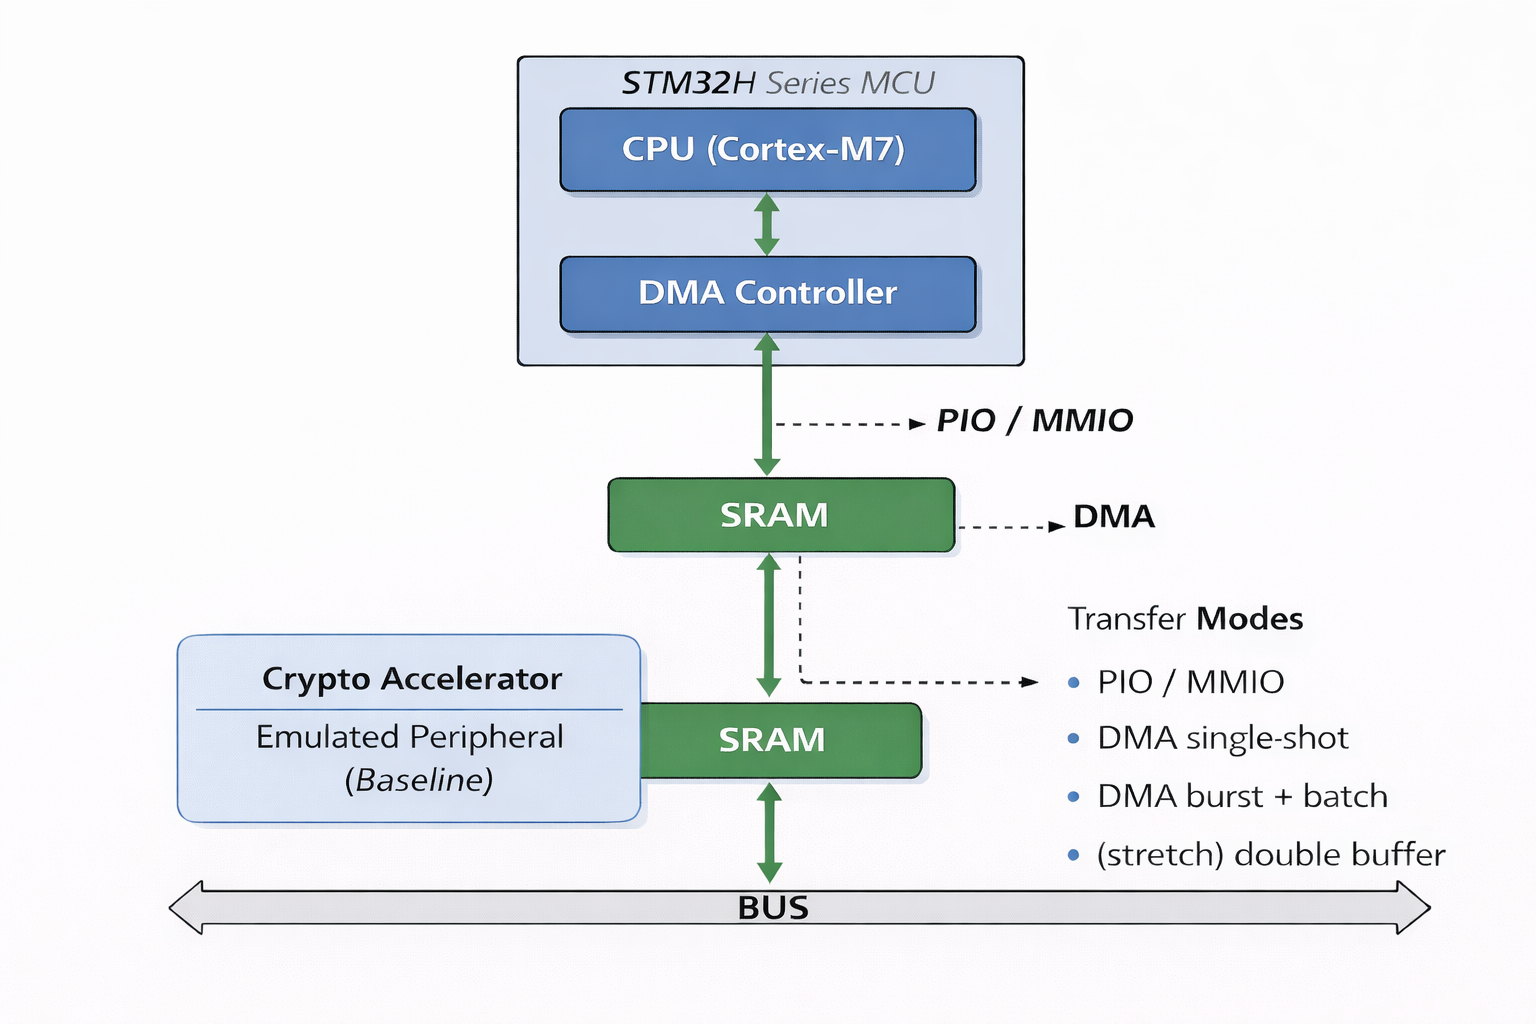
\includegraphics[width=0.78\linewidth]{schematic_1.png}
\end{center}

\PlaceholderBox
  {Motivation / Societal Impact}
  {}
  {
Embedded devices increasingly rely on cryptography for secure boot, authenticated firmware updates, secure communication, and device identity. As stronger cryptographic primitives are adopted, the performance bottleneck often shifts from computation to \emph{system integration}, particularly the efficiency of data transfers between processors, memory, and hardware accelerators.

Inefficient transfer mechanisms waste CPU cycles, increase latency, and raise energy consumption, which directly affects battery-powered and resource-constrained devices. In many real-world systems, a fixed transfer policy is used for simplicity, even though workloads vary significantly between bulk encryption tasks and small control-heavy cryptographic operations.

This project aims to improve the efficiency and robustness of secure embedded systems by developing an adaptive transfer-mode selection mechanism for cryptographic workloads. The proposed approach will benefit developers of IoT devices, industrial control systems, and safety-critical embedded platforms that must maintain strong security guarantees while operating under strict power and latency constraints.

The impact will be evaluated through reductions in end-to-end cryptographic job latency, CPU utilization, and memory-bus traffic. By systematically comparing static transfer strategies with adaptive ones, the project will provide insights into how embedded systems can achieve more efficient integration of cryptographic accelerators without requiring changes to the cryptographic algorithms themselves.
}

\begin{tcolorbox}[proposalbox,title={Related Work / References}]
\vspace{0.5\baselineskip}
\bibliographystyle{ieeetr}
\bibliography{references}
\end{tcolorbox}

\end{document}